\documentclass{beamer}
\usetheme{Madrid}
\usepackage{amsmath,amssymb,amsfonts}
\usepackage{graphicx}
\usepackage{tikz}
\usepackage{pgfplots}
\pgfplotsset{compat=1.17}
\usepackage{siunitx}
\sisetup{output-decimal-marker={.}}

\title{H2 Physics \\ Kinematics: Graphing}
\author{R.F.H.}
\date{\today}

\begin{document}

\begin{frame}
\titlepage
\end{frame}

% --- Question 1 ---
\begin{frame}[shrink=15]{Question 1}
The displacement–time graph for a moving object is shown below.
\begin{center}
\begin{tikzpicture}[scale=1.2]
\draw[->] (0,0) -- (6,0) node[right] {$t$ (s)};
\draw[->] (0,0) -- (0,4) node[above] {$s$ (m)};
\draw[thick] (0,1) -- (2,1) -- (4,3) -- (5,3) -- (6,2);
\node at (0,1) [left] {1};
\node at (2,1) [below] {2};
\node at (4,3) [below] {4};
\node at (5,3) [below] {5};
\node at (6,2) [below] {6};
\end{tikzpicture}
\end{center}
Describe the motion during each time interval and determine the velocity in each segment.
\end{frame}

\begin{frame}[shrink=15]{Solution to Question 1}
\begin{itemize}
    \item 0–2 s: Displacement constant at 1 m → object stationary. Velocity = 0 m/s.
    \item 2–4 s: Displacement increases linearly from 1 m to 3 m → constant velocity.
          \[ v = \frac{3-1}{4-2} = \frac{2}{2} = 1 \text{ m/s} \]
    \item 4–5 s: Displacement constant at 3 m → stationary. Velocity = 0 m/s.
    \item 5–6 s: Displacement decreases linearly from 3 m to 2 m → constant negative velocity.
          \[ v = \frac{2-3}{6-5} = \frac{-1}{1} = -1 \text{ m/s} \]
\end{itemize}
\end{frame}

% --- Question 2 ---
\begin{frame}[shrink=15]{Question 2}
The velocity–time graph of a particle is shown.
\begin{center}
\begin{tikzpicture}[scale=1.2]
\draw[->] (0,0) -- (6,0) node[right] {$t$ (s)};
\draw[->] (0,-2) -- (0,3) node[above] {$v$ (m/s)};
\draw[thick] (0,2) -- (2,2) -- (4,-1) -- (5,-1) -- (6,0);
\node at (0,2) [left] {4};
\node at (2,2) [above] {2};
\node at (4,-1) [below] {4};
\node at (5,-1) [below] {5};
\node at (6,0) [right] {6};
\end{tikzpicture}
\end{center}
Find the acceleration in each phase and the total displacement.
\end{frame}

\begin{frame}[shrink=15]{Solution to Question 2}
Acceleration = gradient of $v$–$t$ graph.
\begin{itemize}
    \item 0–2 s: constant $v=4$ m/s → $a=0$.
    \item 2–4 s: $v$ changes from 4 to $-1$ m/s, $\Delta t=2$ s → $a = \frac{-1-4}{2} = -2.5$ m/s$^2$.
    \item 4–5 s: constant $v=-1$ m/s → $a=0$.
    \item 5–6 s: $v$ changes from $-1$ to 0 m/s, $\Delta t=1$ s → $a = \frac{0-(-1)}{1} = 1$ m/s$^2$.
\end{itemize}
Displacement = area under $v$–$t$ graph (positive above axis, negative below).
\begin{align*}
\text{0–2 s:} & \ 4\times2 = 8 \text{ m} \\
\text{2–4 s:} & \ \frac{1}{2}(4+(-1))\times2 = 3 \text{ m} \quad (\text{trapezoid}) \\
\text{4–5 s:} & \ (-1)\times1 = -1 \text{ m} \\
\text{5–6 s:} & \ \frac{1}{2}(-1+0)\times1 = -0.5 \text{ m} \\
\text{Total} & \ 8+3-1-0.5 = 9.5 \text{ m}
\end{align*}
\end{frame}

% --- Question 3 ---
\begin{frame}[shrink=15]{Question 3}
The acceleration–time graph of a particle starting from rest is shown.
\begin{center}
\begin{tikzpicture}[scale=1.2]
\draw[->] (0,0) -- (6,0) node[right] {$t$ (s)};
\draw[->] (0,-2) -- (0,3) node[above] {$a$ (m/s$^2$)};
\draw[thick] (0,2) -- (2,2) -- (4,-1) -- (6,-1);
\node at (0,2) [left] {2};
\node at (2,2) [above] {2};
\node at (4,-1) [below] {4};
\node at (6,-1) [below] {6};
\end{tikzpicture}
\end{center}
Sketch the velocity–time graph for $t=0$ to $t=6$ s.
\end{frame}

\begin{frame}[shrink=15]{Solution to Question 3}
Velocity is the integral of acceleration. Starting from rest ($v=0$ at $t=0$).
\begin{itemize}
    \item 0–2 s: constant $a=2$ m/s$^2$ → $v$ increases linearly: $v = 2t$. At $t=2$, $v=4$ m/s.
    \item 2–4 s: constant $a=-1$ m/s$^2$ → $v$ decreases linearly from 4 m/s. At $t=4$, $v = 4 + (-1)\times2 = 2$ m/s.
    \item 4–6 s: constant $a=-1$ m/s$^2$ → $v$ continues decreasing linearly. At $t=6$, $v = 2 + (-1)\times2 = 0$ m/s.
\end{itemize}
Sketch:
\begin{center}
\begin{tikzpicture}[scale=1.2]
\draw[->] (0,0) -- (6,0) node[right] {$t$ (s)};
\draw[->] (0,0) -- (0,5) node[above] {$v$ (m/s)};
\draw[thick] (0,0) -- (2,4) -- (4,2) -- (6,0);
\node at (2,4) [above] {4};
\node at (4,2) [below] {2};
\end{tikzpicture}
\end{center}
\end{frame}

% --- Question 4 ---
\begin{frame}[shrink=15]{Question 4}
The displacement–time graph of an object moving in a straight line is given by $s = 2t^2 + 3t + 1$ (SI units).
\begin{enumerate}
    \item Find the velocity at $t=2$ s.
    \item Find the acceleration.
    \item Sketch the $v$–$t$ and $a$–$t$ graphs for $0 \le t \le 3$ s.
\end{enumerate}
\end{frame}

\begin{frame}[shrink=15]{Solution to Question 4}
\begin{enumerate}
    \item Velocity $v = \frac{ds}{dt} = 4t + 3$. At $t=2$, $v = 4(2)+3 = 11$ m/s.
    \item Acceleration $a = \frac{dv}{dt} = 4$ m/s$^2$ (constant).
    \item $v$–$t$: straight line from $(0,3)$ to $(3,15)$. $a$–$t$: horizontal line at $a=4$.
\end{enumerate}
\begin{center}
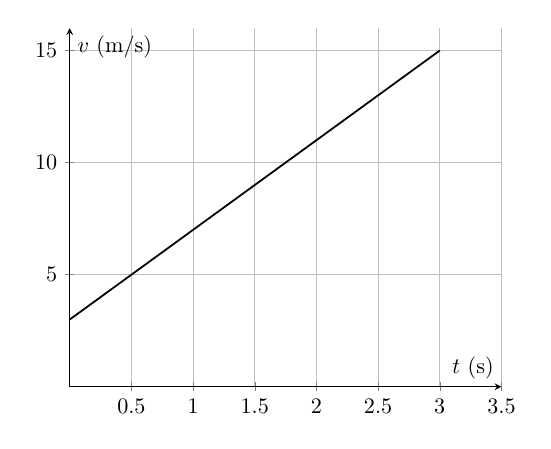
\begin{tikzpicture}[scale=0.8]
\begin{axis}[axis lines=middle, xlabel={$t$ (s)}, ylabel={$v$ (m/s)}, xmin=0, xmax=3.5, ymin=0, ymax=16, grid=both]
\addplot[domain=0:3, thick] {4*x+3};
\end{axis}
\end{tikzpicture}
\qquad
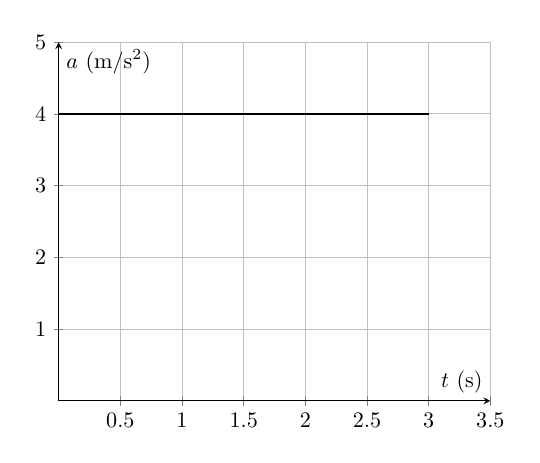
\begin{tikzpicture}[scale=0.8]
\begin{axis}[axis lines=middle, xlabel={$t$ (s)}, ylabel={$a$ (m/s$^2$)}, xmin=0, xmax=3.5, ymin=0, ymax=5, grid=both]
\addplot[domain=0:3, thick] {4};
\end{axis}
\end{tikzpicture}
\end{center}
\end{frame}

% --- Question 5 ---
\begin{frame}[shrink=15]{Question 5}
The velocity–time graph of a train is shown.
\begin{center}
\begin{tikzpicture}[scale=1]
\draw[->] (0,0) -- (10,0) node[right] {$t$ (s)};
\draw[->] (0,-1) -- (0,5) node[above] {$v$ (m/s)};
\draw[thick] (0,0) -- (3,4) -- (7,4) -- (9,0);
\node at (3,4) [above] {3};
\node at (7,4) [above] {7};
\node at (9,0) [below] {9};
\end{tikzpicture}
\end{center}
Describe the motion during each phase and calculate the total distance travelled.
\end{frame}

\begin{frame}[shrink=15]{Solution to Question 5}
\begin{itemize}
    \item 0–3 s: Constant acceleration from rest to 4 m/s. $a = (4-0)/3 = 1.33$ m/s$^2$.
    \item 3–7 s: Constant velocity 4 m/s.
    \item 7–9 s: Constant deceleration from 4 m/s to 0. $a = (0-4)/2 = -2$ m/s$^2$.
\end{itemize}
Distance = area under $v$–$t$ graph:
\begin{align*}
\text{0–3 s: triangle} &\ \frac12 \times 3 \times 4 = 6 \text{ m} \\
\text{3–7 s: rectangle} &\ 4 \times 4 = 16 \text{ m} \\
\text{7–9 s: triangle} &\ \frac12 \times 2 \times 4 = 4 \text{ m} \\
\text{Total} &\ 6+16+4 = 26 \text{ m}
\end{align*}
\end{frame}

% --- Question 6 ---
\begin{frame}[shrink=15]{Question 6}
A car starts from rest, accelerates uniformly at $2$ m/s$^2$ for $5$ s, then travels at constant speed for $10$ s, and finally decelerates uniformly at $4$ m/s$^2$ until it stops. Sketch the velocity–time graph and determine the total distance travelled.
\end{frame}

\begin{frame}[shrink=15]{Solution to Question 6}
Phase 1: $v = at = 2\times5 = 10$ m/s at $t=5$ s. Distance $s_1 = \frac12 \times 5 \times 10 = 25$ m.
Phase 2: constant $v=10$ m/s for $10$ s → $s_2 = 10\times10 = 100$ m.
Phase 3: deceleration $a=-4$ m/s$^2$ from $10$ m/s to $0$: time $t_3 = v/a = 10/4 = 2.5$ s. Distance $s_3 = \frac12 \times 2.5 \times 10 = 12.5$ m.
Total distance = $25+100+12.5 = 137.5$ m.
\begin{center}
\begin{tikzpicture}[scale=0.8]
\draw[->] (0,0) -- (20,0) node[right] {$t$ (s)};
\draw[->] (0,0) -- (0,12) node[above] {$v$ (m/s)};
\draw[thick] (0,0) -- (5,10) -- (15,10) -- (17.5,0);
\node at (5,10) [above] {5};
\node at (15,10) [above] {15};
\node at (17.5,0) [below] {17.5};
\end{tikzpicture}
\end{center}
\end{frame}

% --- Question 7 ---
\begin{frame}[shrink=15]{Question 7}
The graph shows the velocity of a cyclist.
\begin{center}
\begin{tikzpicture}[scale=1]
\draw[->] (0,0) -- (8,0) node[right] {$t$ (s)};
\draw[->] (0,-3) -- (0,3) node[above] {$v$ (m/s)};
\draw[thick] (0,2) -- (2,2) -- (4,-2) -- (6,-2) -- (7,0);
\node at (0,2) [left] {4};
\node at (2,2) [above] {2};
\node at (4,-2) [below] {4};
\node at (6,-2) [below] {6};
\node at (7,0) [below] {7};
\end{tikzpicture}
\end{center}
Find the total displacement and the total distance travelled.
\end{frame}

\begin{frame}[shrink=15]{Solution to Question 7}
Displacement = area above axis minus area below axis.
\begin{itemize}
    \item 0–2 s: rectangle $4\times2 = 8$ m.
    \item 2–4 s: line from $(2,4)$ to $(4,-2)$: slope = $(-2-4)/(2) = -3$. Equation $v = 4 -3(t-2)$. Area = $\int_2^4 (4 -3(t-2)) dt = \int_2^4 (10 -3t) dt = [10t - \frac{3}{2}t^2]_2^4 = (40 - 24) - (20 -6) = 16 -14 = 2$ m.
    \item 4–6 s: constant $v=-2$ m/s, area = $-2\times2 = -4$ m.
    \item 6–7 s: triangle from $-2$ to $0$, area = $\frac12 \times 1 \times (-2) = -1$ m.
\end{itemize}
Displacement = $8 + 2 -4 -1 = 5$ m.
Distance = sum of absolute areas: $8 + 2 + 4 + 1 = 15$ m.
\end{frame}

% --- Question 8 ---
\begin{frame}[shrink=15]{Question 8}
The displacement–time graph of a particle is shown. Indicate the intervals where velocity is positive, negative, or zero.
\begin{center}
\begin{tikzpicture}[scale=1]
\draw[->] (0,0) -- (8,0) node[right] {$t$};
\draw[->] (0,0) -- (0,5) node[above] {$s$};
\draw[thick] plot[smooth, tension=0.7] coordinates {(0,2) (1,3) (2,3) (3,2) (4,2.5) (5,2) (6,0) (7,0.5) (8,1)};
\end{tikzpicture}
\end{center}
\end{frame}

\begin{frame}[shrink=15]{Solution to Question 8}
Velocity is positive when $s$ increases, negative when $s$ decreases, zero when slope is horizontal.
\begin{itemize}
    \item 0–1: increasing → positive
    \item 1–2: constant → zero
    \item 2–3: decreasing → negative
    \item 3–4: increasing → positive
    \item 4–5: decreasing → negative
    \item 5–6: decreasing steeply → negative
    \item 6–7: increasing → positive
    \item 7–8: increasing → positive
\end{itemize}
\end{frame}

% --- Question 9 ---
\begin{frame}[shrink=15]{Question 9}
Two cars A and B start from the same point. Their velocity–time graphs are shown.
\begin{center}
\begin{tikzpicture}[scale=1]
\draw[->] (0,0) -- (8,0) node[right] {$t$ (s)};
\draw[->] (0,-2) -- (0,5) node[above] {$v$ (m/s)};
\draw[thick,blue] (0,2) -- (4,4) -- (8,4);
\draw[thick,red] (0,0) -- (4,2) -- (8,0);
\node[blue] at (7,4.5) {A};
\node[red] at (7,0.5) {B};
\end{tikzpicture}
\end{center}
Determine the time at which they have the same velocity and the time at which they meet again.
\end{frame}

\begin{frame}[shrink=15]{Solution to Question 9}
\begin{itemize}
    \item Velocity equations:
          \begin{align*}
              \text{A: } & v_A = 2 + 0.5t \quad (0 \le t \le 4), \quad v_A = 4 \quad (t \ge 4) \\
              \text{B: } & v_B = 0.5t \quad (0 \le t \le 4), \quad v_B = 4 - 0.5t \quad (t \ge 4)
          \end{align*}
          Setting $v_A = v_B$:
          \begin{itemize}
              \item For $t < 4$: $2 + 0.5t = 0.5t \Rightarrow 2 = 0$, impossible.
              \item For $t \ge 4$: $4 = 4 - 0.5t \Rightarrow 0.5t = 0 \Rightarrow t = 0$, not valid.
          \end{itemize}
          Hence they never have the same velocity.
    \item Displacement equations:
          \begin{align*}
              s_A &= 
              \begin{cases}
                  2t + 0.25t^2, & t \le 4 \\
                  4t - 4, & t \ge 4
              \end{cases} \\
              s_B &= 
              \begin{cases}
                  0.25t^2, & t \le 4 \\
                  4t - 0.25t^2 - 8, & t \ge 4
              \end{cases}
          \end{align*}
          Setting $s_A = s_B$:
          \begin{itemize}
              \item For $t \le 4$: $2t + 0.25t^2 = 0.25t^2 \Rightarrow 2t = 0 \Rightarrow t = 0$.
              \item For $t \ge 4$: $4t - 4 = 4t - 0.25t^2 - 8 \Rightarrow -4 = -0.25t^2 - 8 \Rightarrow 0.25t^2 = -4$, no real solution.
          \end{itemize}
          Thus they meet only at $t=0$ (start).
\end{itemize}
\end{frame}

% --- Question 10 ---
\begin{frame}[shrink=15]{Question 10 (Challenging)}
The acceleration of a particle moving along a straight line is given by $a = 4 - 2t$ (SI units) for $0 \le t \le 4$ s. At $t=0$, $v=2$ m/s and $s=0$.
\begin{enumerate}
    \item Find the velocity as a function of time.
    \item Find the displacement as a function of time.
    \item Sketch the $v$–$t$ and $s$–$t$ graphs.
\end{enumerate}
\end{frame}

\begin{frame}[shrink=15]{Solution to Question 10}
\begin{enumerate}
    \item $a = \frac{dv}{dt} = 4 - 2t$ → integrate: $v = \int (4-2t) dt = 4t - t^2 + C$. Using $v(0)=2$ gives $C=2$. So $v(t) = 4t - t^2 + 2$.
    \item $v = \frac{ds}{dt}$ → $s = \int (4t - t^2 + 2) dt = 2t^2 - \frac{t^3}{3} + 2t + D$. $s(0)=0$ gives $D=0$. So $s(t) = 2t^2 - \frac{t^3}{3} + 2t$.
    \item $v$–$t$ is a downward parabola with vertex at $t=2$ (since $dv/dt = 4-2t=0$ gives $t=2$). $v(2)=4(2)-4+2=6$ m/s. $v(4)=16-16+2=2$ m/s. $s$–$t$ is cubic.
\end{enumerate}
\begin{center}
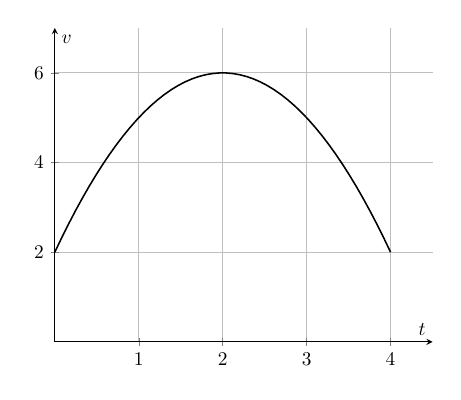
\begin{tikzpicture}[scale=0.7]
\begin{axis}[axis lines=middle, xlabel={$t$}, ylabel={$v$}, xmin=0, xmax=4.5, ymin=0, ymax=7, grid=both]
\addplot[domain=0:4, samples=50, thick] {4*x - x^2 + 2};
\end{axis}
\end{tikzpicture}
\qquad
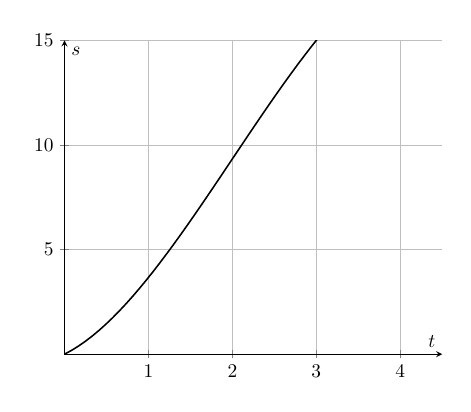
\begin{tikzpicture}[scale=0.7]
\begin{axis}[axis lines=middle, xlabel={$t$}, ylabel={$s$}, xmin=0, xmax=4.5, ymin=0, ymax=15, grid=both]
\addplot[domain=0:4, samples=50, thick] {2*x^2 - x^3/3 + 2*x};
\end{axis}
\end{tikzpicture}
\end{center}
\end{frame}

% --- Question 11 ---
\begin{frame}[shrink=15]{Question 11}
The velocity–time graph of a particle is shown. Sketch the corresponding acceleration–time graph.
\begin{center}
\begin{tikzpicture}[scale=1]
\draw[->] (0,0) -- (8,0) node[right] {$t$};
\draw[->] (0,-2) -- (0,4) node[above] {$v$};
\draw[thick] (0,3) -- (2,1) -- (4,1) -- (6,3) -- (8,3);
\end{tikzpicture}
\end{center}
\end{frame}

\begin{frame}[shrink=15]{Solution to Question 11}
Acceleration is gradient of $v$–$t$:
\begin{itemize}
    \item 0–2 s: gradient = $(1-3)/2 = -1$ m/s$^2$ → constant $a=-1$.
    \item 2–4 s: gradient = 0 → $a=0$.
    \item 4–6 s: gradient = $(3-1)/2 = 1$ m/s$^2$ → constant $a=1$.
    \item 6–8 s: gradient = 0 → $a=0$.
\end{itemize}
\begin{center}
\begin{tikzpicture}[scale=1]
\draw[->] (0,0) -- (8,0) node[right] {$t$};
\draw[->] (0,-2) -- (0,2) node[above] {$a$};
\draw[thick] (0,-1) -- (2,-1) -- (2,0) -- (4,0) -- (4,1) -- (6,1) -- (6,0) -- (8,0);
\node at (1,-1) [below] {$-1$};
\node at (5,1) [above] {$1$};
\end{tikzpicture}
\end{center}
\end{frame}

% --- Question 12 ---
\begin{frame}[shrink=15]{Question 12}
The graph shows the displacement of two runners A and B starting from the same point.
\begin{center}
\begin{tikzpicture}[scale=1]
\draw[->] (0,0) -- (8,0) node[right] {$t$ (s)};
\draw[->] (0,0) -- (0,5) node[above] {$s$ (m)};
\draw[thick,blue] (0,0) -- (4,3) -- (8,3);
\draw[thick,red] (0,0) -- (2,2) -- (6,4) -- (8,4);
\node[blue] at (7,3.5) {A};
\node[red] at (7,4.5) {B};
\end{tikzpicture}
\end{center}
Determine the time when B overtakes A and their velocities at that instant.
\end{frame}

\begin{frame}[shrink=15]{Solution to Question 12}
Displacement functions:
\begin{align*}
    s_A &= 
    \begin{cases}
        \frac{3}{4}t, & 0 \le t \le 4 \\
        3, & t \ge 4
    \end{cases} \\
    s_B &= 
    \begin{cases}
        t, & 0 \le t \le 2 \\
        \frac12 t + 1, & 2 \le t \le 6 \\
        4, & t \ge 6
    \end{cases}
\end{align*}
Setting $s_A = s_B$ for $t \le 2$: $\frac34 t = t \Rightarrow t=0$.
For $2 \le t \le 4$: $\frac34 t = \frac12 t + 1 \Rightarrow \frac14 t = 1 \Rightarrow t=4$ s.
At $t=4$, $s_A = s_B = 3$ m.
For $t > 4$, $s_A = 3$, $s_B > 3$ (since $s_B$ increases to 4), so B is always ahead after $t=4$. Thus they meet only at $t=4$, but B was ahead before $t=4$ and remains ahead after; therefore B never overtakes A—they are just momentarily together. Velocities at $t=4$:
\begin{itemize}
    \item $v_A = \frac{3}{4} = 0.75$ m/s (constant for $t<4$).
    \item $v_B = \frac12$ m/s (from $2 \le t \le 6$).
\end{itemize}
Thus at $t=4$, $v_A = 0.75$ m/s, $v_B = 0.5$ m/s.
\end{frame}

% --- Question 13 ---
\begin{frame}[shrink=15]{Question 13 (Relative motion)}
Two cars P and Q move along the same straight road. Their velocity–time graphs are shown.
\begin{center}
\begin{tikzpicture}[scale=1]
\draw[->] (0,0) -- (8,0) node[right] {$t$ (s)};
\draw[->] (0,-2) -- (0,5) node[above] {$v$ (m/s)};
\draw[thick,blue] (0,3) -- (2,3) -- (4,5) -- (6,5) -- (8,1);
\draw[thick,red] (0,1) -- (4,1) -- (6,3) -- (8,3);
\node[blue] at (7,2) {P};
\node[red] at (7,3.5) {Q};
\end{tikzpicture}
\end{center}
At $t=0$, they are alongside. Find the time when they are again alongside.
\end{frame}

\begin{frame}[shrink=15]{Solution to Question 13}
Compute displacement functions by integrating velocity.
For P:
\begin{align*}
    &0-2: s_P = 3t \\
    &2-4: v_P = 3 + (t-2) = t+1, \quad s_P = 6 + \int_2^t (t+1) dt = 0.5t^2 + t + 2 \\
    &4-6: v_P = 5, \quad s_P = 14 + 5(t-4) = 5t -6 \\
    &6-8: v_P = 5 -2(t-6) = 17 -2t, \quad s_P = 24 + \int_6^t (17-2\tau) d\tau = 17t - t^2 -42
\end{align*}
For Q:
\begin{align*}
    &0-4: s_Q = t \\
    &4-6: v_Q = 1 + (t-4) = t-3, \quad s_Q = 4 + \int_4^t (t-3) dt = 0.5t^2 -3t + 8 \\
    &6-8: v_Q = 3, \quad s_Q = 8 + 3(t-6) = 3t -10
\end{align*}
Set $s_P = s_Q$ for $t \ge 6$ (since for earlier intervals they are not equal except at $t=0$):
\begin{align*}
    17t - t^2 -42 = 3t -10 \Rightarrow -t^2 + 14t -32 = 0 \Rightarrow t^2 -14t +32 = 0 \\
    t = \frac{14 \pm \sqrt{196 -128}}{2} = \frac{14 \pm \sqrt{68}}{2} = \frac{14 \pm 8.246}{2}
\end{align*}
$t = 11.123$ s or $t = 2.877$ s (but $t=2.877$ is not in $t \ge 6$). Thus they meet again at $t \approx 11.1$ s.
\end{frame}

% --- Question 14 ---
\begin{frame}[shrink=15]{Question 14 (Projectile)}
A ball is thrown vertically upward with initial speed $20$ m/s. Sketch the velocity–time and acceleration–time graphs for the entire flight until it returns to the thrower's hand. Take upward as positive.
\end{frame}

\begin{frame}[shrink=15]{Solution to Question 14}
Upward positive, $g = -9.81$ m/s$^2$ constant.
Velocity: $v = 20 - 9.81t$. Graph is straight line from $(0,20)$ to $(t_{\text{top}},0)$ where $t_{\text{top}} = 20/9.81 \approx 2.04$ s. Then continues negative until $t_{\text{total}} = 2t_{\text{top}} \approx 4.08$ s, at which $v = -20$ m/s.
Acceleration: constant at $-9.81$ m/s$^2$.
\begin{center}
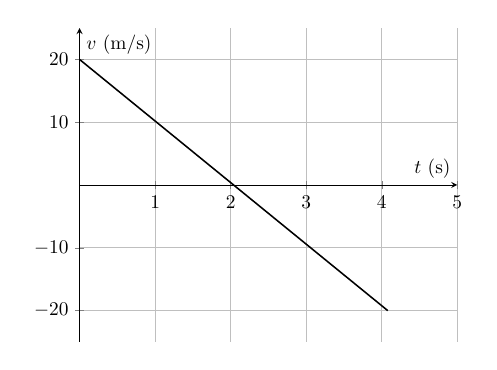
\begin{tikzpicture}[scale=0.7]
\begin{axis}[axis lines=middle, xlabel={$t$ (s)}, ylabel={$v$ (m/s)}, xmin=0, xmax=5, ymin=-25, ymax=25, grid=both]
\addplot[domain=0:4.08, thick] {20 - 9.81*x};
\end{axis}
\end{tikzpicture}
\qquad
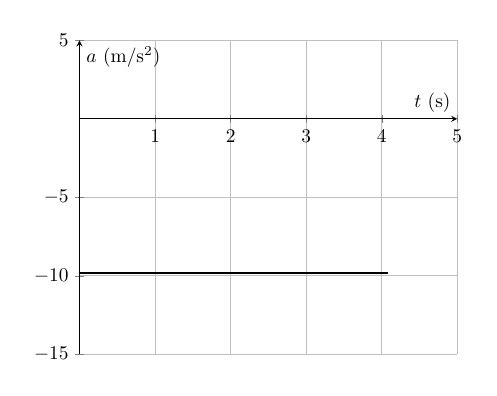
\begin{tikzpicture}[scale=0.7]
\begin{axis}[axis lines=middle, xlabel={$t$ (s)}, ylabel={$a$ (m/s$^2$)}, xmin=0, xmax=5, ymin=-15, ymax=5, grid=both]
\addplot[domain=0:4.08, thick] {-9.81};
\end{axis}
\end{tikzpicture}
\end{center}
\end{frame}

% --- Question 15 ---
\begin{frame}[shrink=15]{Question 15 (Terminal velocity)}
A skydiver jumps from a high platform. Initially she accelerates downward, but air resistance increases with speed until she reaches terminal velocity. Sketch qualitatively the $v$–$t$ and $a$–$t$ graphs.
\end{frame}

\begin{frame}[shrink=15]{Solution to Question 15}
$v$–$t$: starts from rest, increases with decreasing slope (since acceleration decreases), asymptotically approaching terminal velocity $v_T$.
$a$–$t$: starts at $g$, decreases to 0 as terminal velocity is approached.
\begin{center}
\begin{tikzpicture}[scale=0.8]
\draw[->] (0,0) -- (6,0) node[right] {$t$};
\draw[->] (0,0) -- (0,4) node[above] {$v$};
\draw[thick] (0,0) to[out=70,in=180] (5,3);
\draw[dashed] (5,3) -- (6,3) node[right] {$v_T$};
\end{tikzpicture}
\qquad
\begin{tikzpicture}[scale=0.8]
\draw[->] (0,0) -- (6,0) node[right] {$t$};
\draw[->] (0,0) -- (0,4) node[above] {$a$};
\draw[thick] (0,3) to[out=0,in=180] (5,0.2);
\node at (0,3) [left] {$g$};
\end{tikzpicture}
\end{center}
\end{frame}

\end{document}